 \documentclass[10pt, table, dvipsnames,xcdraw, handout ]{beamer}
\usetheme[progressbar=frametitle]{metropolis}
\usepackage{appendixnumberbeamer}
\usetikzlibrary{arrows.meta, positioning, quotes}
\usepackage[shortlabels]{enumitem}
\usepackage{xcolor}
\usepackage{mathtools}

\usepackage{cancel}

\newcommand\hcancel[2][black]{\setbox0=\hbox{$#2$}%
\rlap{\raisebox{.45\ht0}{\textcolor{#1}{\rule{\wd0}{1pt}}}}#2} 


\usepackage{booktabs}
\usepackage[scale=2]{ccicons}

\usepackage{pgfplots}
\usepgfplotslibrary{dateplot}

\usepackage{xspace}
\newcommand{\themename}{\textbf{\textsc{metropolis}}\xspace}
\newcommand{\cb}{\cellcolor{blue!25}}


% Notation:
\newcommand{\cT}{\ensuremath{\mathcal{T}}}
\newcommand{\cD}{\ensuremath{\mathcal{D}}}
\newcommand{\cX}{\ensuremath{\mathcal{X}}}
\newcommand{\cY}{\ensuremath{\mathcal{Y}}}
\newcommand{\cZ}{\ensuremath{\mathcal{Z}}}
\newcommand{\cH}{\ensuremath{\mathcal{H}}}

\newcommand{\bR}{\ensuremath{\mathbb{R}}}
\newcommand{\bN}{\ensuremath{\mathbb{N}}}
\newcommand{\bP}{\ensuremath{\mathbb{P}}}
\newcommand{\bT}{\ensuremath{\mathbb{T}}}
\newcommand{\bL}{\ensuremath{\mathbb{L}}}

\newcommand{\bfX}{\ensuremath{\mathbf{X}}}
\newcommand{\bfY}{\ensuremath{\mathbf{Y}}}
\newcommand{\bfy}{\ensuremath{\mathbf{y}}}

% Tikz seys
\tikzset{cross/.style={cross out, draw, 
         minimum size=2*(#1-\pgflinewidth), 
         inner sep=0pt, outer sep=0pt}}

\title{Machine Learning I}
\subtitle{Lecture 3: Linear Regression}
% \date{\today}
\date{}
\author{Nathaniel Bade}
\institute{Northeastern University Department of Mathematics}
% \titlegraphic{\hfill\includegraphics[height=1.5cm]{logo.pdf}}

\begin{document}

\maketitle

\begin{frame}{Table of contents}
  \setbeamertemplate{section in toc}[sections numbered]
  \tableofcontents[hideallsubsections]
\end{frame}


%%%%%%%%%%%%%% PAC Learning %%%%%%%%%%%%%% 



\section{Least Squares for Linear Models}



\begin{frame}[fragile]{Linear Models: Definition}
  \begin{minipage}[t][0.5\textheight][t]{\textwidth}
	\centering \includegraphics[height=0.5\textheight]{L7Regression1.png} 
  \end{minipage}
  \vfill
\begin{minipage}[t][0.5\textheight][t]{\textwidth}
A \textbf{linear regression model} is a model of data fitting that assume that the regression function $E(Y|X)$ is linear in the inputs $X_1,\ldots, X_p$,
$$
Y = \beta_0 + X_1\beta_1 +\ldots + X_p\beta_p +  \epsilon
$$ 
and uses the residual sum of squares $RSS(\beta)$ as a loss function. Here $\epsilon$ is a random variable with $E[\epsilon] = 0$.
\end{minipage}
\end{frame}


\begin{frame}[fragile]{Linear Models: Definition}
  \begin{minipage}[t][0.5\textheight][t]{\textwidth}
	\centering \includegraphics[height=0.5\textheight]{L7Regression2.png} 
  \end{minipage}
  \vfill
\begin{minipage}[t][0.5\textheight][t]{\textwidth}
A \textbf{linear regression model} is a model of data fitting that assume that the regression function $E(Y|X)$ is linear in the inputs $X_1,\ldots, X_p$,
$$
Y = \beta_0 + X_1\beta_1 +\ldots + X_p\beta_p + \epsilon
$$ 
and uses the residual sum of squares $RSS(\beta)$ as a loss function. Here $\epsilon$ is a random variable with $E[\epsilon] = 0$.
\end{minipage}
\end{frame}



\begin{frame}[fragile]{Linear Models: Definition}
  \begin{minipage}[t][0.5\textheight][t]{\textwidth}
	\centering \includegraphics[height=0.5\textheight]{L7Regression1.png} 
  \end{minipage}
  \vfill
\begin{minipage}[t][0.5\textheight][t]{\textwidth}
In vector form, we add a constant term $X = (1,X_1,\ldots, X_p)$ and let $\beta$ be a $p+1$ vector including $\beta_0$:
$$
Y = \beta_0 + X_1\beta_1 +\ldots + X_p\beta_p \epsilon = X^T\beta + \epsilon\,,
$$ 
where again we uses the residual sum of squares $RSS(\beta)$ as a loss function.
\end{minipage}
\end{frame}



\begin{frame}[fragile]{Linear Models: ERM Solution}
  \begin{minipage}[t][0.5\textheight][t]{\textwidth}
	\centering \includegraphics[height=0.5\textheight]{L7Regression2.png} 
  \end{minipage}
  \vfill
\begin{minipage}[t][0.5\textheight][t]{\textwidth}
Given the $N\times (p+1)$ matrix $\bfX$ of $N$ input data points $x_i$ and a vector $\bfy$ of the $N$ corresponding labels $y_i$, we saw that 
$$
RSS(\beta) = \sum_{i=1}^N(y_i - x_i^T)^2 = (\bfy - \bfX\beta)^T(\bfy - \bfX\beta)
$$
is minimized by $\hat{\beta} = (\bfX^T\bfX)^{-1}\bfX^T\bfy$.
\end{minipage}
\end{frame}




\begin{frame}[fragile]{Linear Models: Goodness of Fit}
  \begin{minipage}[t][0.5\textheight][t]{\textwidth}
	\centering \includegraphics[height=0.5\textheight]{L7Regression3.png} 
  \end{minipage}
  \vfill
\begin{minipage}[t][0.5\textheight][t]{\textwidth}
We now turn our attention to quantifying the goodness of our fit. We would like to answer two questions:
\begin{itemize}
\item How much do we expect $\hat{f}$ to change if we draw different data from the same distribution?
\item Which parameters correspond to statistically significant features?
\end{itemize}
\end{minipage}
\end{frame}




\begin{frame}[fragile]{Linear Models: Pointwise Variance}
  \begin{minipage}[t][0.5\textheight][t]{\textwidth}
	\centering \includegraphics[height=0.5\textheight]{L7Regression5.png} 
  \end{minipage}
  \vfill
\begin{minipage}[t][0.5\textheight][t]{\textwidth}
To the second question: when fitting multivariate (multi-feature) linear models, one of our main goals is to understand which parameters most directly control the labeling. \pause\newline  

For a multilinear model, the coefficients $\beta$ give some measure of correlation, but we still need to investigate what exactly these variables mean, what constitute expected and unexpected values.

\end{minipage}
\end{frame}




\begin{frame}[fragile]{Example Data}
In the lecture we're going to use as an example a data set of undergraduate confidence in admission to graduate school. The data has 8 input features and 1 output feature\newline 

\textbf{Data Sample:}\newline 


\begin{tabular}{lllllllll}
\hline
\textbf{Serial No.} & \textbf{GRE Score} & \multicolumn{1}{c}{\textbf{TOEFL Score}} & \textbf{University Rating} \\ \hline
1                   & 337                & 118                                      & 4                         \\
2                   & 324                & 107                                      & 4                         \\
3                   & 316                & 104                                      & 3                         
\end{tabular}


\begin{tabular}{lllllllll}
\hline
\textbf{SOP} & \textbf{LOR} & \textbf{CGPA} & \textbf{Research} & \textbf{Chance of Admit} \\ \hline
4.5          & 4.5          & 9.65          & 1                 & 0.92                     \\
4.0          & 4.5          & 8.87          & 1                 & 0.76                     \\
3.0          & 3.5          & 8.00          & 1                 & 0.72                    
\end{tabular}

\end{frame}




\begin{frame}[fragile]{Example Data}
The features of the data are

\begin{itemize}
\item[] \textbf{Serial No.} \pause
\item[] \textbf{GRE Score:} Out of 340.\pause
\item[] \textbf{TOEFL Score:} Out of 120. \pause
\item[] \textbf{University Ranking:} Out of 5.\pause
\item[] \textbf{SOP:} Statement of purpose strength out of 5.\pause
\item[] \textbf{LOR:} Letter of recommendation strength out of 5.\pause
\item[] \textbf{CGPA:} Undergraduate GPA out of 10.\pause
\item[] \textbf{Research:} Research experience 0 or 1.\pause
\item[] \textbf{Chance of Admit:} Chance of admission.\pause
\end{itemize}
Note: This data claims to be self reported, it is not authoritative. 


\end{frame}


\begin{frame}[fragile]
\vspace{1em}
	\centering \includegraphics[height=1\textheight]{L7Data1.png} 
\end{frame}




\begin{frame}[fragile]{Linear Models: Parameter Variance}
The fit parameter $\hat \beta_i$ in the linear model 
$$
\hat Y = X^T\hat \beta
$$
describes the expected correlation between the $i$'th feature and the chance of admission. \pause Before we discuss the fit of the model, we will discuss the quantitative meaning of the parameters and understand what the data informs us an expected for the parameters $\hat \beta_i$. 

In particular, we want to understand quantitatively when a parameter value $\hat \beta_i$ is statistically significant. \pause Statistically, this mean we want expressions for the $p$-values and confidence intervals for the $\hat\beta_i$ that can be computed from the data set. \pause

Mathematically, this boils down to understanding variance of $\hat \beta_i$ as a function of the input data $\bfX$ and $\bfy$. 
\end{frame}



\section{Variance of Parameters}


\begin{frame}[fragile]{Review: Confidence Intervals}
First, lets quickly recall the confidence interval paradigm in statistics. Suppose we want to estimate the mean $\mu$ of a distribution from a data set $x_i$, $i=1,\ldots, N$ drawn from the distribution. Our \textbf{point estimate} for the mean is 
$$
\hat{m} = \frac{1}{N}\sum_{i=1}^N x_i\,.
$$
One way to quantify the accuracy of this estimate is to compute a \textbf{confidence interval}, or \textbf{interval estimate} for the statistic $\hat{m}$. \pause

To compute a confidence interval we have to make some assumptions about the distribution of the statistic over the space of different draws from background distribution. 

\end{frame}



\begin{frame}[fragile]{Review: Confidence Intervals}
For computations of the mean, we often invoke the \textbf{Central Limit Theorem} (CLT) to assume that the distribution of test statistics is drawn from a Normal Distribution:
$$
\mathcal{N}(\sigma^2, \mu)  = \mathcal{N}(X|\sigma^2, \mu) = \frac{1}{\sqrt{2\pi \sigma^2}}e^{-\frac12\left(\frac{X-\mu}{\sigma}\right)^2}\,.
$$\pause
The CLT roughly states that for $X_j$, $j=1,\ldots, p$ drawn independently from any distributions with expected value $\mu$ and variance $\sigma^2$, then 
$$
\hat{m}_p = \frac{X_1+\ldots +X_p}{p}\,,\,\, \Rightarrow \,\, \frac{\hat{m}_p - \mu}{\sigma/\sqrt{p}} \xrightarrow{p} \mathcal{N}\left(1, 0\right) \,,
$$
that is that $m_p$ is approximately normally distributed over samples from the dataset when $p$ is large. 
\end{frame}



\begin{frame}[fragile]{Review: Confidence Intervals}
Given a specific test statistic $\hat{m}$, the $C\%$ confidence interval $I_C$ is the interval in which $C\%$ of the computations of $\hat{m}$ from random draws of the data will lie. This interval should contain $\hat{m}$ with a high probability, no matter what the value of $\mu$ is. \pause 

Formally, for any statistic $\theta = f(x_1,\ldots, x_N)$ the $1-\alpha$ confidence interval $I$ is a set such that
$$
P_{\theta} (\theta \in I)  \geq 1-\alpha\,.
$$
That is $I$ traps $\theta$ with probability $1-\alpha$. 
\end{frame}





\begin{frame}[fragile]{Review: Confidence Intervals}
  \begin{minipage}[t][0.5\textheight][t]{\textwidth}
	\centering \includegraphics[height=0.5\textheight]{L7StandError2.png} 
  \end{minipage}
  \vfill
\begin{minipage}[t][0.5\textheight][t]{\textwidth}
By the CLT, $Z = \frac{\hat{m} - \mu}{\sigma/\sqrt{p}}$ is distributed by the \textbf{standard normal distribution} $Z\sim\mathcal{N}(1,0)$. It is standard to use $Z$ to parameterize this distribution. Then, if 95\% of the distribution $Z$ is captured in the interval $[-z_{95}, z_{95}]$, than we expect that 95\% of the sampled $\hat{m}$ will fall in the interval
$$
I_{95} = \left[
\hat{m} - z_{95}\frac{\sigma}{\sqrt{p}},\hat{m} + z_{95}\frac{\sigma}{\sqrt{p}}
\right]\,.
$$
\end{minipage}
\end{frame}



\begin{frame}[fragile]{Review: Confidence Intervals}
  \begin{minipage}[t][0.5\textheight][t]{\textwidth}
	\centering \includegraphics[height=0.5\textheight]{L7StandError2.png} 
  \end{minipage}
  \vfill
\begin{minipage}[t][0.5\textheight][t]{\textwidth}
In summary, the process for constructing a confidence interval is
\begin{itemize}
\item \textbf{(1)} Construct a test statistic $S$
\item \textbf{(2)} Determine the distribution $\mathcal{D}$ for $S$ over different samples (possibly up to assumptions on data distribution).
\item \textbf{(3)} Find an interval $I_C$ that captures C\% of the draws from $\mathcal{D}$. Generally this will be centered $S$, but it need not be. 
\end{itemize}
\end{minipage}
\end{frame}





\begin{frame}[fragile]{Linear Models: Definition}
  \begin{minipage}[t][0.5\textheight][t]{\textwidth}
	\centering \includegraphics[height=0.5\textheight]{L5Linear1.png} 
  \end{minipage}
  \vfill
\begin{minipage}[t][0.5\textheight][t]{\textwidth}
Given our linear model
$$
Y = \beta_0 + X_1\beta_1 +\ldots + X_p\beta_p + \epsilon = X^T\beta + \epsilon\,,
$$ 
fit by minimizing RSS, we want to compute confidence intervals for each of the parameters $\beta_j$. 
\end{minipage}
\end{frame}




\begin{frame}[fragile]{Linear Classifier with Noise}
  \begin{minipage}[t][0.5\textheight][t]{\textwidth}
	  \centering \includegraphics[height=0.5\textheight]{L5Linear1.png}
  \end{minipage}
  \vfill
  \begin{minipage}[t][0.5\textheight][t]{\textwidth}
Suppose that we know that the relationship between $X$ and $Y$ is almost linear
$$
Y = f_*(X) = X^T\beta_* + \epsilon\,,
$$\pause
where $\beta_*$ denotes the actual weights and $\epsilon$ is a random variable drawn from a normal distribution with $E[\epsilon] = 0$ and variance $\sigma^2$.	
\end{minipage}
\end{frame}


\begin{frame}[fragile]{Linear Classifier with Noise}
  \begin{minipage}[t][0.5\textheight][t]{\textwidth}
	  \centering \includegraphics[height=0.5\textheight]{L5Linear2.png}
  \end{minipage}
  \vfill
  \begin{minipage}[t][0.5\textheight][t]{\textwidth}
The variance in the fit parameters $\hat{\beta}$ over draws of $N$ data points $\bfX$ is
$$
\textbf{Var}(\hat{\beta}) = \text{Var}_{\epsilon}\big( (\bfX^T\bfX)^{-1}\bfX^T\bfy \big)\,.
$$
We would like to derive an explicit expression for $\textbf{Var}(\hat{\beta})$ in terms of $\bfX$, $\bfy$ and $\sigma^2$.
\end{minipage}
\end{frame}





\begin{frame}[fragile]{Linear Classifier with Noise}
Recall that for a $p$-vector $X$ of random variables, $\text{Var}(X)$ is a $p\times p$ matrix with $jk$'th entry given by the covariance
$$
\text{Var}(X)_{jk} = \text{Cov}(X_j,X_k) = E[(X_j-E[X_j])(X_k - E[X_k])\,.
$$\pause
For a set of datapoint $x_i\in \mathbb{R}^p$ collected into the matrix $\mathbf{X}$ let the sample mean of the $j$'th feature be $\hat{m}_j = E[\mathbf{x}_j]$. One can compute the sample covariance from datapoints as
$$
\text{Cov}(\mathbf{x}_j,\mathbf{x}_k)  = \frac1N \sum_{i=1}^N (\mathbf{X}_{ij} - \hat{m}_j)(\mathbf{X}_{ik} - \hat{m}_k)\,.
$$
All together, $\text{Var}(X)=E[(X - E[X])(X - E[X])^T]$.
\end{frame}





\begin{frame}[fragile]{Variance of Linear Transform}
For vector $\epsilon$ of i.i.d. random variables each with variance $\sigma^2_\epsilon$, and a matrix $A$,
$$
\text{Var}(A\epsilon) = \sigma^2_\epsilon A A^T\,.
$$\pause
This follow from the definition of the (co)variance matrix $\text{Var}(\epsilon)=E[(\epsilon - E[\epsilon])(\epsilon - E[\epsilon])^T]$:
\begin{align*}
\action<+->{\text{Var}(A\epsilon)  &= E[(A\epsilon - E[A\epsilon])(A\epsilon - E[A\epsilon])^T] && \text{Definition of Var.}}
\\
\action<+->{&=A \, E[(\epsilon - E[\epsilon])(\epsilon - E[\epsilon])^T] \, A^T && \text{$A$ constant}}
\\
\action<+->{&=A \, \text{Var}(\epsilon) \, A^T&& \text{Definition of Var.}}
\\
\action<+->{&=A (\sigma_\epsilon^2 I ) A^T && \text{$\epsilon$ i.i.d.}}
\\
\action<+->{&= \sigma_\epsilon^2A A^T &&}
\end{align*}
\action<+->{The second the last line come from the fact that i.i.d. variables are uncorrelated, and so all off diagonal entries are 0.}

\end{frame}






\begin{frame}[fragile]{Linear Models: Parameter Variance}
The formula 
\begin{align}
\text{Var}(A\epsilon) = \sigma^2_\epsilon A A^T\,.
\end{align}
allow us to make a direct derivation of the parameter variance. Assume that the input points are fixed and the variance comes only from the labels. Then
\begin{align*}
\action<+->{\text{Var}_{\epsilon}(\hat \beta) &=\text{Var}_{\epsilon}\big( (\bfX^T\bfX)^{-1}\bfX^T\bfy \big)  && \text{Definition of  $\hat \beta$,}}
\\
\action<+->{  &=\text{Var}_{\epsilon}\big( (\bfX^T\bfX)^{-1}\bfX^T(\bfX\beta_* + \epsilon) \big)  && \text{Definition of  $\bfy$,} }
\\
\action<+->{  &=\text{Var}_{\epsilon}\big(\beta_* + (\bfX^T\bfX)^{-1}\bfX^T\epsilon \big)  &&  \text{Distribution,}}
\\
\action<+->{  &=\text{Var}_{\epsilon}\big((\bfX^T\bfX)^{-1}\bfX^T\epsilon \big)  &&  \text{Var(const) = 0,}}
\\
\action<+->{  &=\sigma^2_\epsilon\, \big((\bfX^T\bfX)^{-1}\bfX^T \big) \big((\bfX^T\bfX)^{-1}\bfX^T \big)^T  && \text{(1) Above,}}
\\
\action<+->{  &=\sigma^2_\epsilon\, (\bfX^T\bfX)^{-1}  && \text{Multiplication.}}
\end{align*}
\end{frame}





\begin{frame}[fragile]{Linear Models: Parameter Variance}
The variation of the parameters is then a $p+1\times p+1$ matrix
$$
\text{Var}(\hat \beta) = \sigma^2_\epsilon\, (\bfX^T\bfX)^{-1} \,,
$$
 with each term scaled by the variance of the noise parameter (recall that $\bfX$ contains a column of 1's).\pause 

Note, that unlike for the variance matrix of the i.i.d. variables $\epsilon$ in the computation for $\text{Var}(A\epsilon)$, we expect there to be correlation between the $\beta_i$'s, and there will almost certainly be non-diagonal terms in the matrix. 
\end{frame}




\begin{frame}[fragile]
For example, the variance in the parameters for the admission dataset is 
	\centering \includegraphics[height=1\textheight]{L7BCovar.png} 
\end{frame}




\section{Confidence Intervals for Coefficients }



\begin{frame}[fragile]{Estimating Total Variance}
In practice, the variance $\sigma^2_\epsilon$ of the random variable isn't given to us but must be estimated from the data. The variance is typically estimated by
$$
\hat \sigma^2 = \frac{1}{N-p-1}\sum_{i=1}^N(y_i - \hat y_i)^2 = \frac{RSS(\hat \beta)}{N-p-1}\,.
$$\pause
The factor of $N-p-1$ in the denominator makes $\hat \sigma$ into an \textbf{unbiased estimator}, in the sense that 
$$
E[\hat \sigma^2] = \sigma^2\,.
$$
\end{frame}





\begin{frame}[fragile]{Linear Models: Parameter Variance}
The intuition here is roughly that just as the sample variance for one parameter is corrected by 
$$
\bar{s} = \frac{1}{n-1}\sum_{i=1}^n(y_i-\bar{y})^2\,,
$$
the sample variance for our $p+1$ parameters will be corrected by a $p+1$ shift:
$$
\hat \sigma^2 = \frac{1}{N-p-1}\sum_{i=1}^N(y_i - \hat y_i)^2 = \frac{1}{N-p-1}\sum_{i=1}^N(r_i - E[r_i])^2\,,
$$
where $r_i = y_i - \hat{y}_i$ is leftover error in the fit at each datapoint, and $E[r_i] $ is expected to vanish for $RSS$.
\end{frame}




\begin{frame}[fragile]{Linear Models: Parameter Variance}
Since 
$$
\text{Var}_\epsilon(\hat \beta) = \sigma^2_\epsilon\, (\bfX^T\bfX)^{-1} \,,
$$
(and linear regression is an unbiased predictor, $E_{\cT}[\hat \beta] = \beta_*$), if we assume that $\epsilon$ is normally distribution, that is $\epsilon \sim N(0,\sigma^2_\epsilon)$, then the the linear parameters are normally distributed around the true solution $\beta_*$ with covariance matrix $\sigma^2_\epsilon\, (\bfX^T\bfX)^{-1}$. 
$$
\hat \beta \sim N(\beta_*, \sigma^2_\epsilon\, (\bfX^T\bfX)^{-1} )\,.
$$
\end{frame}



\begin{frame}[fragile]{Linear Models: Parameter Variance}
The standard deviation for each coefficient can be read off the diagonal entries of the covariance matrix $\sigma^2_\epsilon\, (\bfX^T\bfX)^{-1}$,
$$
\hat \sigma_i = \sqrt{\text{Var}(\hat \beta_i)} = \sigma_\epsilon \sqrt{(\bfX^T\bfX)^{-1}_{ii}}\,,
$$
where $(\bfX^T\bfX)^{-1}_{ii}$ is the $i$'th diagonal entry of $(\bfX^T\bfX)^{-1}$. \pause\newline

To test the hypothesis that $\beta_i = 0$, that is the $i$'th feature has no bearing on the outcome, we write the standardized $z$ score
\begin{flalign*}
\boxed{\,\text{Z-Score of $\beta_i$}\,} \hspace{2em} z_i \approx \frac{\hat \beta_i}{\hat\sigma_i} = \frac{\hat \beta_i}{\sigma_\epsilon \sqrt{(\bfX^T\bfX)^{-1}_{ii}}}\,.&&
\end{flalign*}
Practically speaking, if $|z_i|>2$ and $N$ is large, the chance that $(\beta_*)_i = 0$ is less than 5\%.
\end{frame}




\begin{frame}[fragile]{Z-scores}
  \begin{minipage}[t][0.5\textheight][t]{\textwidth}
	\centering \includegraphics[height=0.5\textheight]{L7StandError2.png} 
  \end{minipage}
  \vfill
\begin{minipage}[t][0.5\textheight][t]{\textwidth}
Given a linear distribution with normal noise, the $z_i\sim \mathcal{N}(1,0)$ are distributed according to a standard normal distribution. The 95\% CI around each $\beta$ is then 
$$
I_{95} = \left[\hat \beta_i - z_{95}\sigma \sqrt{(\bfX^T\bfX)^{-1}_{ii}}, \hat \beta_i  + z_{95}\sigma \sqrt{(\bfX^T\bfX)^{-1}_{ii}} \right]
$$
\end{minipage}
\end{frame}









\section{Fit, standard error and $z$-score on example data}






\begin{frame}[fragile]{T-score For Application Data}
Example: The fit coefficients for the admissions data with their standard errors. 
\begin{table}[]
\begin{tabular}{llll}
\hline
\textbf{Variable} & \textbf{coef} & \multicolumn{1}{c}{\textbf{std err}} & \textbf{z} \\ \hline
const             & 0.3257        & 0.014                                & 24.024     \\
Serial No.        & 0.0722        & 0.012                                & 5.884      \\
GRE Score         & 0.0979        & 0.032                                & 3.077      \\
TOEFL Score       & 0.0994        & 0.032                                & 3.144      \\
University Rating & 0.0433        & 0.020                                & 2.133      \\
SOP               & 0.0078        & 0.023                                & 0.336      \\
LOR               & 0.0663        & 0.023                                & 2.860      \\
CGPA              & 0.3077        & 0.041                                & 7.418      \\
Research          & 0.0217        & 0.008                                & 2.587     
\end{tabular}
\end{table}
\end{frame}



\begin{frame}[fragile]{T-score For Application Data}
We find the highest significance for the constant $\beta_0$, with the second highest being for GPA. 
\begin{table}[]
\begin{tabular}{llll}
\hline
\textbf{Variable} & \textbf{coef} & \multicolumn{1}{c}{\textbf{std err}} & \textbf{z} \\ \hline
\rowcolor[HTML]{FFCCC9} 
const             & 0.3257        & 0.014                                & 24.024     \\
Serial No.        & 0.0722        & 0.012                                & 5.884      \\
GRE Score         & 0.0979        & 0.032                                & 3.077      \\
TOEFL Score       & 0.0994        & 0.032                                & 3.144      \\
University Rating & 0.0433        & 0.020                                & 2.133      \\
SOP               & 0.0078        & 0.023                                & 0.336      \\
LOR               & 0.0663        & 0.023                                & 2.860      \\
\rowcolor[HTML]{FFCCC9} 
CGPA              & 0.3077        & 0.041                                & 7.418      \\
Research          & 0.0217        & 0.008                                & 2.587     
\end{tabular}
\end{table}
\end{frame}



\begin{frame}[fragile]{T-score For Application Data}
Surprisingly, we also find a high significance for the coefficient of the Serial No. \pause This is suspicious, and we see that the coefficient itself is small. 
\begin{table}[]
\begin{tabular}{llll}
\hline
\textbf{Variable} & \textbf{coef} & \multicolumn{1}{c}{\textbf{std err}} & \textbf{z} \\ \hline
const             & 0.3257        & 0.014                                & 24.024     \\
\rowcolor[HTML]{FFCCC9} 
Serial No.        & 0.0722        & 0.012                                & 5.884      \\
GRE Score         & 0.0979        & 0.032                                & 3.077      \\
TOEFL Score       & 0.0994        & 0.032                                & 3.144      \\
University Rating & 0.0433        & 0.020                                & 2.133      \\
SOP               & 0.0078        & 0.023                                & 0.336      \\
LOR               & 0.0663        & 0.023                                & 2.860      \\
CGPA              & 0.3077        & 0.041                                & 7.418      \\
Research          & 0.0217        & 0.008                                & 2.587     
\end{tabular}
\end{table}
\end{frame}


\begin{frame}[fragile]{T-score For Application Data}
Surprisingly, we also find a high significance for the coefficient of the Serial No. This is suspicious, and we see that the coefficient itself is small. 
\begin{table}[]
\begin{tabular}{llll}
\hline
\textbf{Variable} & \textbf{coef} & \multicolumn{1}{c}{\textbf{std err}} & \textbf{z} \\ \hline
\rowcolor[HTML]{FFCCC9} 
Serial No.        & 0.0722        & 0.012                                & 5.884      \\
\end{tabular}
\end{table}
This high significance mostly likely comes from the fact that the correlation is so low that the standard error is low. It means that the model may be over fitting, using a effectively random parameter to generate a tighter fit to the specific dataset. \pause Such terms tend to lead to a higher variance in our models, and should be eliminated if possible. If we compute the correlation matrix we will see that Serial No. is effectively uncorrelated with the acceptance percentage. 
\end{frame}





\begin{frame}[fragile]{Correlation}
	\centering \includegraphics[height=1\textheight]{L7Data2.png} 
\end{frame}




\begin{frame}[fragile]{Correlation}
Lets breakdown what we're seeing on the previous slide:\pause
\begin{itemize}
\item[] \textbf{Serial No.} is basically uncorrelated with anything. \pause
\item[] \textbf{Admit} is highly correlated with \textbf{CGPA}, \textbf{TOEFL Score} and \textbf{GRE Score}\pause
\item[] \textbf{Research} has a lowish correlation with \textbf{Admit}, but also with everything else.  
\end{itemize}
\end{frame}

\begin{frame}[fragile]{Correlation}
	\centering \includegraphics[height=1\textheight]{L7Data2.png} 
\end{frame}



\begin{frame}[fragile]{T-score For Application Data}
Going back to our fit, we find that \textbf{CGPA} has a highly significant coefficient, but \textbf{TOEFL} and \textbf{GRE} are much more similar to \textbf{research}. Why could this be?
\begin{table}[]
\begin{tabular}{llll}
\hline
\textbf{Variable} & \textbf{coef} & \multicolumn{1}{c}{\textbf{std err}} & \textbf{z} \\ \hline
const             & 0.3257        & 0.014                                & 24.024     \\
Serial No.        & 0.0722        & 0.012                                & 5.884      \\
GRE Score         & 0.0979        & 0.032                                & 3.077      \\
TOEFL Score       & 0.0994        & 0.032                                & 3.144      \\
University Rating & 0.0433        & 0.020                                & 2.133      \\
SOP               & 0.0078        & 0.023                                & 0.336      \\
LOR               & 0.0663        & 0.023                                & 2.860      \\
CGPA              & 0.3077        & 0.041                                & 7.418      \\
Research          & 0.0217        & 0.008                                & 2.587     
\end{tabular}
\end{table}
\end{frame}


\begin{frame}[fragile]{T-score For Application Data}
What about \textbf{SOP}? The correlation with \textbf{Admit} is .68 but the $z$ value of the coefficient is utterly insignificant. Why could that be?
\begin{table}[]
\begin{tabular}{llll}
\hline
\textbf{Variable} & \textbf{coef} & \multicolumn{1}{c}{\textbf{std err}} & \textbf{z} \\ \hline
const             & 0.3257        & 0.014                                & 24.024     \\
Serial No.        & 0.0722        & 0.012                                & 5.884      \\
GRE Score         & 0.0979        & 0.032                                & 3.077      \\
TOEFL Score       & 0.0994        & 0.032                                & 3.144      \\
University Rating & 0.0433        & 0.020                                & 2.133      \\
SOP               & 0.0078        & 0.023                                & 0.336      \\
LOR               & 0.0663        & 0.023                                & 2.860      \\
CGPA              & 0.3077        & 0.041                                & 7.418      \\
Research          & 0.0217        & 0.008                                & 2.587     
\end{tabular}
\end{table}
\end{frame}


\begin{frame}[fragile]{T-score For Application Data}
The answer is probably internal correlation. The model gets the best fit by using \textbf{CGPA} to account for general trends and the other variables, highly correlated with it, to fine tune the fit. 
\begin{table}[]
\begin{tabular}{llll}
\hline
\textbf{Variable} & \textbf{coef} & \multicolumn{1}{c}{\textbf{std err}} & \textbf{z} \\ \hline
const             & 0.3257        & 0.014                                & 24.024     \\
Serial No.        & 0.0722        & 0.012                                & 5.884      \\
GRE Score         & 0.0979        & 0.032                                & 3.077      \\
TOEFL Score       & 0.0994        & 0.032                                & 3.144      \\
University Rating & 0.0433        & 0.020                                & 2.133      \\
SOP               & 0.0078        & 0.023                                & 0.336      \\
LOR               & 0.0663        & 0.023                                & 2.860      \\
CGPA              & 0.3077        & 0.041                                & 7.418      \\
Research          & 0.0217        & 0.008                                & 2.587     
\end{tabular}
\end{table}
This could be useful, or it lead to overfitting. 
\end{frame}




\begin{frame}[fragile]{T-score For Application Data}
For comparison, lets recall the variance matrix for the parameters
\begin{table}[]
\begin{tabular}{llll}
\hline
\textbf{Variable} & \textbf{coef} & \multicolumn{1}{c}{\textbf{std err}} & \textbf{z} \\ \hline
const             & 0.3257        & 0.014                                & 24.024     \\
Serial No.        & 0.0722        & 0.012                                & 5.884      \\
GRE Score         & 0.0979        & 0.032                                & 3.077      \\
TOEFL Score       & 0.0994        & 0.032                                & 3.144      \\
University Rating & 0.0433        & 0.020                                & 2.133      \\
SOP               & 0.0078        & 0.023                                & 0.336      \\
LOR               & 0.0663        & 0.023                                & 2.860      \\
CGPA              & 0.3077        & 0.041                                & 7.418      \\
Research          & 0.0217        & 0.008                                & 2.587     
\end{tabular}
\end{table}

\end{frame}


\begin{frame}[fragile]{Variance for Admission}
Varaiance Matrix $\text{Var}(\hat\beta) = \hat\sigma^2 (\bfX^T\bfX)^{-1}$
	\centering \includegraphics[height=.9\textheight]{L7BCovar.png} 
\end{frame}



\begin{frame}[fragile]{Variance for Admission}
These values are probably low due to to the relatively large sample size and the small number of parameters. Note that we we see that \textbf{CGPA} has a negative covariance with \textbf{GRE} and \textbf{TOEFL}. \pause

This is what we would expect, since all three are highly correlated we would expect a lessening of fit by \textbf{CGPA} could be compensated for by a tightening of the fit on \textbf{GRE} or \textbf{TOEFL}. 
\end{frame}











\section{Feature Selection via Statistical Significance}


\begin{frame}[fragile]{Overfitting}
  \begin{minipage}[t][0.5\textheight][t]{\textwidth}
	\centering \raisebox{0.1\height}{\includegraphics[width=0.45\textwidth]{L3Overfit1.png} }
	\includegraphics[width=0.45\textwidth]{L3Overfit2.png} 
  \end{minipage}
  \vfill
\begin{minipage}[t][0.5\textheight][t]{\textwidth}
One of the goals of preliminary data analysis is to determine if variables are \textbf{redundant} or \textbf{random}, since both can lead to additional unnecessary computations, or overfitting. For example, assume that $X_1$ and $X_2$ are linearly correlated, that is $X_2 = mX_1$. Then all of the datapoints lie on the hyperplane $X_2 = mX_1$ and the problem is simply $p-1$ dimensional. 
\end{minipage}
\end{frame}




\begin{frame}[fragile]{Overfitting}
  \begin{minipage}[t][0.5\textheight][t]{\textwidth}
	\centering \raisebox{0.15\height}{\includegraphics[width=0.45\textwidth]{L3Overfit3.png} }
	\includegraphics[width=0.45\textwidth]{L3Overfit4.png} 
  \end{minipage}
  \vfill
\begin{minipage}[t][0.5\textheight][t]{\textwidth}
Notice that any rotation of this plane that includes the horizontal fit line will \emph{also} be a best fit line for the data.
\end{minipage}
\end{frame}









\begin{frame}[fragile]{Overfitting}
  \begin{minipage}[t][0.5\textheight][t]{\textwidth}
	\centering \raisebox{0.1\height}{\includegraphics[width=0.45\textwidth]{L3Overfit5.png} }
	\includegraphics[width=0.45\textwidth]{L3Overfit6.png} 
  \end{minipage}
  \vfill
\begin{minipage}[t][0.5\textheight][t]{\textwidth}
On the other hand, assume that $X_2 = mX_1 + \epsilon$. The data points no longer lie on a hyperplane, but clustered very close to one. The linear function will then effectively fit to $X_1$, and then use $X_2$ to try to capture the other points, possibly resulting in absurdly high $\beta_2$. If we genuinely think $X_1$ and $X_2$ capture different data, this is a feature; if we think say $X_1$ and $X_2$ differ by sampling error or encoding error we may have over fit.
\end{minipage}
\end{frame}





\begin{frame}[fragile]{Overfitting}
  \begin{minipage}[t][0.5\textheight][t]{\textwidth}
	\centering \raisebox{0.1\height}{\includegraphics[width=0.45\textwidth]{L3Overfit5.png} }
	\includegraphics[width=0.45\textwidth]{L3Overfit6.png} 
  \end{minipage}
  \vfill
\begin{minipage}[t][0.5\textheight][t]{\textwidth}
If $X_1$ has no correlation with the labels, we need to worry about overfitting as well. A truly uncorrelated variable at best gives us no information and so is a computational hazard and at worst may allow a linear classifier to over fit, since by a linear transform of the data $(X_1, mX_1 + \epsilon) \to (X_1, \epsilon)$. In short, random features increase model variance. 
\end{minipage}
\end{frame}


\begin{frame}[fragile]{Overfitting}
One of the main challenges of predictive statistics is figuring out how to identify and reduce model variance. 

\begin{itemize}
\item[] A probability approach will use the $F$-statistic to compare significance of dropping groupings of variables from the model.\pause
\item[] A more computational approach will iterate over all possible subsets of features, pulling out the smallest number of features that give a consistent error. \pause
\item[] A more machine learning approach asks us to modify the loss function, attempting to punish the algorithm for incorrect coefficients.\pause
\end{itemize}
We will explore all of these options in the lectures and labs, starting with a review of $F$-statistics.
\end{frame}



\begin{frame}[fragile]{F-statistic}
  \begin{minipage}[t][0.5\textheight][t]{\textwidth}
	\centering \includegraphics[height=0.5\textheight]{L7F-distribution.png} 
  \end{minipage}
  \vfill
\begin{minipage}[t][0.5\textheight][t]{\textwidth}
The $F_{d1,d2}$ distribution is used the compare the ratio of sample variances (normalized by the true variances) for normally distributed random variables, where $d1$ and $d2$ are the respective number of degrees of freedom in each sample. \pause Formally, 
$$
F \sim \frac{s_1^2}{\sigma_1^2}\big/ \frac{s_2^2}{\sigma_2^2}\,.
$$
\end{minipage}


\end{frame}



\begin{frame}[fragile]{F-statistic}
Consider two models, models A and B, with model A fitting a subset of the parameters of model B. Assume model A has $p_A$ parameters and model B has $p_B>p_A$ parameters. \pause

The $F$-statistic measure the relative sum squared of residuals between the two models, which in turn allows us to use the $F$ distribution to test the level of significance. \pause 

Computing $RSS$ on all the test data, the $F$-statistic is defined as 
$$
F = \frac{(RSS_A - RSS_B)/(p_B-p_A)}{RSS_B/(N-p_B-1)}\,.
$$
The $F$ statistic measures if the removed $\beta_j$ are indeed 0. 
\end{frame}




\begin{frame}[fragile]{F-statistic}
Under the Gaussian assumption for $\epsilon$ and the null hypothesis that the smaller model (model A) is the true model, the $F$-statistic will have a 
$$
F\sim F_{p_B-p_A,N-p_B - 1}
$$
distribution. \pause The $F$ distribution assess the statistical significance of setting the $\beta_j$ dropped from model A to 0. If significance is found, we should assume the variables are not redundant. \pause\newline

\textbf{Exercise:} Show that that square of the $z$-score $z_j$ is the $F$ statistics of dropping the single variable $X_i$ from the model. 
\end{frame}



\begin{frame}[fragile]{T-score For Application Data}
For example, we could consider dropping the insignificant \textbf{SOP} and the significant but uncorrelated \textbf{Serial No.} from the classifier.   
\begin{table}[]
\begin{tabular}{llll}
\hline
\textbf{Variable} & \textbf{coef} & \multicolumn{1}{c}{\textbf{std err}} & \textbf{z} \\ \hline
const             & 0.3257        & 0.014                                & 24.024     \\
Serial No.        & 0.0722        & 0.012                                & 5.884      \\
GRE Score         & 0.0979        & 0.032                                & 3.077      \\
TOEFL Score       & 0.0994        & 0.032                                & 3.144      \\
University Rating & 0.0433        & 0.020                                & 2.133      \\
SOP               & 0.0078        & 0.023                                & 0.336      \\
LOR               & 0.0663        & 0.023                                & 2.860      \\
CGPA              & 0.3077        & 0.041                                & 7.418      \\
Research          & 0.0217        & 0.008                                & 2.587     
\end{tabular}
\end{table}
\end{frame}





\begin{frame}[fragile]{F-statistic}
Comparing this new model to the old model give a test statistics
$$
F = \frac{(RSS_A - RSS_B)/(p_B-p_A)}{RSS_B/(N-p_B-1)}\,.
$$
is
$$
F = \frac{(1.239 - 1.114)/(8-6)}{1.114/(320 - 9)} = 17.45
$$
Checking against $F_{6,311}$, we find that this is highly statistically significant, as we predicted from the standard error. \pause By contrast, the $F$ statistic for just dropping \textbf{SOP} is
$$
F = \frac{(1.114861 - 1.114456)/(8-7)}{1.114/(320 - 9)} = 0.1130 \approx (0.336)^2\,.
$$
Checking against $F_{7,311}$, $F$ is not statistically significant, so we can safely drop it. 
\end{frame}






\begin{frame}[fragile]{F-statistic}
We've come to an impasse: Correlation tells us to drop the feature \textbf{Serial No.} while the F statistic (and the $z_j$ number) tell us it is significant. How do we understand this?

\begin{itemize}
\item There is actually a small but significant correlation between the serial number and the chance of admit, we should not drop the variable but should note this.\pause
\item The linear model is over fitting, we should drop the variable.  \pause
\item The fit is bad enough 
\end{itemize}
\end{frame}




\section{Subset Selection Methods}


\begin{frame}[fragile]{Subset Selection}
There are a few reasons why we might not be satisfied with the least squares estimate. \pause

\begin{itemize}
\item[] \textbf{Prediction accuracy:} Least squares estimates often have low bias at the cost of high variance. One is often able to reduce variance by selectively setting some coefficients to 0.\pause
\item[] \textbf{Interpretive power:} With a large number of related parameters, one often wants to find a small number of predictors with strong, definite effects. You don't have to do quantum mechanics to build a car, and often when looking for the ``big picture" we are willing to sacrifice some granularity.  
\end{itemize}
\end{frame}



\begin{frame}[fragile]{Best Subset Selection}
In best subset selection, we perform a regression on every subset of variables of size $k$ and pick the model with the smallest mean squared error. \pause There are efficient algorithms (for example the \emph{leaps and bounds} procedure) that make this possible for $p$ up to 30 or 40, but the total number of subsets grows exponentially
$$
Pow(\{1,\ldots, k\}) = 2^k\,.
$$\pause
The question becomes how to choose $k$. There are many criteria, typically one uses the smallest model that minimizes the estimates of the expected prediction error. 
\end{frame}


\begin{frame}[fragile]{Best Subset Selection}
  \begin{minipage}[t][0.5\textheight][t]{\textwidth}
	\centering \includegraphics[height=0.45\textheight]{L7Traintest.png} 
  \end{minipage}
  \vfill
\begin{minipage}[t][0.5\textheight][t]{\textwidth}
A common way to evaluate models is to randomly cut the available data into a training set and a test set. The exact percentages of data to use for training and test depend a bit on the problem, but an 80\%-20\% split between training and test data is common.  \pause Here, we see how low variance data fits better to the test set. 
\end{minipage}
\end{frame}


\begin{frame}[fragile]{Best Subset Selection}
  \begin{minipage}[t][0.5\textheight][t]{\textwidth}
	\centering \includegraphics[height=0.45\textheight]{L7Traintest.png} 
  \end{minipage}
  \vfill
\begin{minipage}[t][0.5\textheight][t]{\textwidth}
In best subset selection, we train each of our models on a random 80\% of the training data and then validate on the remaining 20\%. \pause If we have the computational power, we may do this for many random partitions of the data into training and test sets. 
\end{minipage}
\end{frame}



\begin{frame}[fragile]{Best Subset Selection}
For the Student Admissions data, we can perform best subset selection for subsets of all size $k$.\pause\newline

For $k=1$, we are fitting a linear model to only one variable and picking out the best test regression.

\begin{table}[]
\begin{tabular}{lll}
\hline
\textbf{Variable} & \textbf{MSE train} & \textbf{MSE test} \\ \hline
CGPA 	&0.004629 	&0.005665\\
TOEFL Score 	&0.007271 	&0.008874\\
GRE Score  	&0.006701 	&0.009308\\
LOR	&0.011041 	&0.011981\\
University Rating 	&0.009177 	&0.013495\\
SOP	&0.010336 	&0.013964\\
Research	&0.013240 	&0.017531\\
Serial No.	&0.018787 	&0.026214
\end{tabular}
\end{table}
\end{frame}


\begin{frame}[fragile]{Best Subset Selection}
Another common human readable scoring mechanism is the $r^2$ statistic
$$
r^2 = 1 - \frac{\sum_i(y_i - \hat y_i)^2}{\sum_i (y_i - \bar y)^2}
$$
where $r^2 = 1$ is perfect correlation.
\begin{table}[]
\begin{tabular}{lll}
\hline
\textbf{Variable} & \textbf{$r^2$ Train} & \textbf{$r^2$ Test} \\ \hline
CGPA 	&0.780614 	&0.755038\\
GRE Score  	&0.639539 	&0.645389\\
TOEFL Score 	&0.656348 	&0.615228\\
University Rating 	&0.477414 	&0.514386\\
SOP	&0.459257 	&0.453055\\
LOR	&0.536031 	&0.415755\\
Research	&0.321136 	&0.299415\\
Serial No.	&-0.015145 	&0.005851
\end{tabular}
\end{table}
\end{frame}






\begin{frame}[fragile]{Correlation}
	\centering \includegraphics[height=1\textheight]{L7Data2.png} 
\end{frame}



\begin{frame}[fragile]{Best Subset Selection}
  \begin{minipage}[t][0.6\textheight][t]{\textwidth}
	\centering \includegraphics[height=0.6\textheight]{L7SubsetSelection.png} 
  \end{minipage}
  \vfill
\begin{minipage}[t][0.4\textheight][t]{\textwidth}
For $k=1$ the best subset regression matches up with the correlation matrix. As we increase $k$, the training error continuous to drop, but the test error levels out and even starts to rise a bit for $k>5$. 

\end{minipage}


\end{frame}




\begin{frame}[fragile]{Best Subset Selection}
  \begin{minipage}[t][0.6\textheight][t]{\textwidth}
	\centering \includegraphics[height=0.6\textheight]{L7SubsetSelection.png} 
  \end{minipage}
  \vfill
\begin{minipage}[t][0.4\textheight][t]{\textwidth}
It turns out the best subsets use \textbf{GRE}, \textbf{LOR} and \textbf{CGPA}. This may be a little surprising given that coefficient of \textbf{LOR} scored rather middling significance in the full model. Why could this be?

\end{minipage}
\end{frame}




\begin{frame}[fragile]{Forward Subset Selection}
For enough features, the $2^p$ possible subsets of variables becomes computationally expensive. \textbf{Forward subset selection} tries to forge a good path through the forest of parameter choices. \pause

The algorithm starts by fitting the intercept, and then sequentially adds into the model the variable that most improves the fit. The algorithm produces a nested sequence of models and is classified as a \textbf{greedy algorithm} since it makes local optimization choices at each steps instead of global ones. \pause

Forward subset selection has a number of regression steps polynomial in the number of features, and can be made even more efficient with a bit of linear algebra. 
\end{frame}



\begin{frame}[fragile]{Backward Subset Selection}
Backward subset regression starts with the full model and sequentially deletes the predictor with the smallest $z$-score. It can only be used when the data set is larger than the number of features, ie when $N>p$.

Backward subset selection is particularly useful when you expect to have a large number of features contributing to the final fit. 
\end{frame}


\begin{frame}[fragile]{Forward and Backward Subset Selection}
There are two main advantages to forward and backward subset selection:\pause

\begin{itemize}
\item[] \textbf{Computational:} Forward/backward subset selection are more computationally efficient then performing an exhaustive search of all subsets of variables.\pause
\item[] \textbf{Stability:} If we allow our model to select the best subset of the features, we must pay the price of a larger variance. As always, we may be able to afford this, but for small training sets we may be more interested in stability. 
\end{itemize}
We will be implementing these methods over the next (few) labs. 
\end{frame}



\begin{frame}[fragile]{References}
This lecture was adapted primarily from Elements of Statistical Learning, Chapter 3. 

For a good explanation of the proof that $\hat \sigma$ is an unbiased estimator, see

\url{https://stats.stackexchange.com/questions/20227/why-is-rss-distributed-chi-square-times-n-p}

Geogebra and Desmose were used for pictures. 

\end{frame}

\end{document}

\begin{frame}[fragile]{Correlation}
Lets breakdown what we're seeing on the previous slide:\pause
\begin{itemize}
\item[] \textbf{Serial No.} is basically uncorrelated with anything. \pause
\item[] \textbf{Admit} is highly correlated with \textbf{CGPA}, \textbf{TOEFL Score} and \textbf{GRE Score}\pause
\item[] \textbf{Research} has a lowish correlation with \textbf{Admit}, but also with everything else.  
\end{itemize}
\end{frame}

\begin{frame}[fragile]{Correlation}
	\centering \includegraphics[height=1\textheight]{L7Data2.png} 
\end{frame}






\begin{frame}[fragile]{Avoiding Underfitting}
The no free lunch theorem isn't the end of machine learning, it simply asserts that there is no universally best learner for every task. If fact, it implies that we should use any prior knowledge to avoid learners that perform poorly on a distribution. Such prior knowledge can be expressed by restricting the hypothesis class. \pause

But how do we choose this class? On one hand, we want a class that contains a classifier that will return the minimum error. On the other hand, the class of all functions is clearly not learnable so we cant just choose the richest class. 
\end{frame}



\begin{frame}[fragile]{Bias, Variance and Parameters}
  \begin{minipage}[t][0.5\textheight][t]{\textwidth}
	\centering
	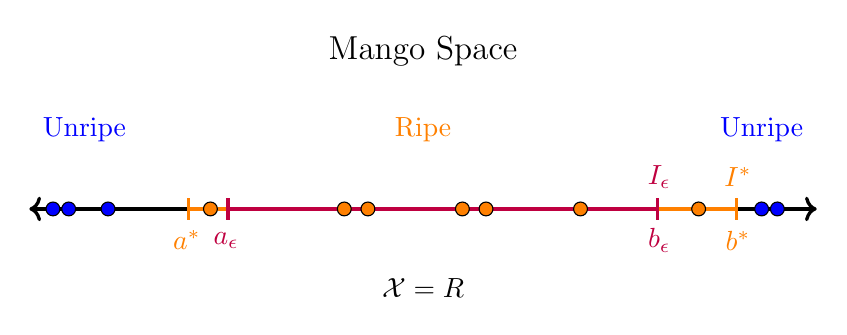
\begin{tikzpicture}
		\draw[<->,very thick] (-5,0) -- (5,0);
		\draw[color = orange, |-|,very thick] (-3,0) -- (4,0);
		\node[color=orange] at (4,.4) {$I^*$};
		\node at (0,2) {\large Mango Space} ;
		\node at (0,-1) {$\mathcal{X} = \mathbb{R}$} ;
		\node [color=blue] at (-4.3,1) {Unripe} ;
		\node [color=blue] at (4.3,1) {Unripe} ;
		\node [color=orange] at (0,1) {Ripe} ;

		\node [color=orange] at (-3,-.4) {$a^*$} ;
		\node [color=orange] at (4,-.4) {$b^*$} ;

		\draw [color=purple, |-|,very thick] (-2.5,0) -- (3,0);
		\node [color=purple] at (3,.4) {$I_\epsilon$} ;
		\node [color=purple] at (-2.5,-.4) {$a_\epsilon$} ;
		\node [color=purple] at (3,-.4) {$b_\epsilon$} ;

%		\draw [color=olive, |-|,very thick] (-3.5,0) -- (2.5,0);
%		\node [color=olive] at (3,.4) {$h_{\mathcal{T}}$} ;



		\node[circle,draw=black, fill=orange, inner sep=0pt,minimum size=5pt] at (2,0) {};
		\node[circle,draw=black, fill=orange, inner sep=0pt,minimum size=5pt] at (-1,0) {};
		\node[circle,draw=black, fill=orange, inner sep=0pt,minimum size=5pt] at (-.7,0) {};
		\node[circle,draw=black, fill=orange, inner sep=0pt,minimum size=5pt] at (.5,0) {};
		\node[circle,draw=black, fill=orange, inner sep=0pt,minimum size=5pt] at (.8,0) {};
		\node[circle,draw=black, fill=orange, inner sep=0pt,minimum size=5pt] at (-2.7,0) {};
		\node[circle,draw=black, fill=orange, inner sep=0pt,minimum size=5pt] at (3.5,0) {};

		\node[circle,draw=black, fill=blue, inner sep=0pt,minimum size=5pt] at (-4.5,0) {};
		\node[circle,draw=black, fill=blue, inner sep=0pt,minimum size=5pt] at (-4,0) {};
		\node[circle,draw=black, fill=blue, inner sep=0pt,minimum size=5pt] at (-4.7,0) {};
		\node[circle,draw=black, fill=blue, inner sep=0pt,minimum size=5pt] at (4.3,0) {};
		\node[circle,draw=black, fill=blue, inner sep=0pt,minimum size=5pt] at (4.5,0) {};
	\end{tikzpicture}
  \end{minipage}
  \vfill
  \begin{minipage}[t][0.5\textheight][t]{\textwidth}
Lets understand this visually.
$$
Err(x_0) = \sigma_\epsilon^2 + [E_\cT[\hat f(x_0)] - f(x_0)]^2 + E_\cT\big[ \hat{f}(x_0) - E_\cT[\hat{f}(x_0)] \big]^2\,.
$$\pause
Consider a data set, 
\end{minipage}
\end{frame}


\begin{frame}[fragile]{Point Variance of Linear Predictor}
Since $x_0^T  (\bfX^T\bfX)^{-1}\bfX^T\epsilon$ is a vector, squaring it is the same as multiply by its transpose. \pause This allow us to write
\begin{align*}
\action<+->{\textbf{Var} &= E_\cT\big[(\,x_0^T  (\bfX^T\bfX)^{-1}\bfX^T\epsilon\,)^2\big] && \text{From before,}}
\\
\action<+->{  &=   E_\cT\big[(\,x_0^T  (\bfX^T\bfX)^{-1}\bfX^T\epsilon\,)(\,x_0^T  (\bfX^T\bfX)^{-1}\bfX^T\epsilon\,)^T\big]  && }
\\
\action<+->{  &=   E_\cT\big[(\,x_0^T  (\bfX^T\bfX)^{-1}\bfX^T\epsilon\,)(\epsilon^T \bfX (\bfX^T\bfX)^{-1} \,x_0)\big] &&  }
\\
\action<+->{  &= (\,x_0^T  (\bfX^T\bfX)^{-1}\bfX^T) E_\cT[\epsilon\epsilon^T] (\bfX (\bfX^T\bfX)^{-1} x_0)  &&\bfX,\,x_0\,\text{const,}}
\\
\action<+->{  &=  (\,x_0^T  (\bfX^T\bfX)^{-1}\bfX^T)\,(\sigma_\epsilon^2 I)\, (\bfX (\bfX^T\bfX)^{-1} x_0)  && \text{Def. of Var,} }
\\
\action<+->{  &=  \sigma^2_\epsilon \, \,x_0^T  (\bfX^T\bfX)^{-1}x_0  && \text{Simplify.} }
\end{align*}
\action<+->{The variance is proportional to the variance in the random variable. But how do we understand the matrix $(\bfX^T\bfX)^{-1}$?}
\end{frame}


























